\documentclass[../../main.tex]{subfiles}



\begin{document}
\section{Quicksort and Concurrency}
\subsection{Comparing quicksort implementations}
\subsubsection{Benchmarking environment}
The benchmarks were performed on the following system:

\begin{description}[style=nextline, labelwidth=4.8cm, labelindent=0cm, leftmargin=5cm, font=\normalfont\bfseries]
    \item[Operating System:] Ubuntu 24.04.1 LTS
    \item[RAM:] 32 GB
    \item[CPU:] AMD Ryzen 5 5600G with Radeon Graphics (6 Cores, 2 Threads per Core)
    \item[Compiler:] gcc version 13.2.0
\end{description}


\newpage
\subsubsection{Running time comparison with different numbers of threads}
Here are the results when running the sorting algorithms with varying numbers of threads:

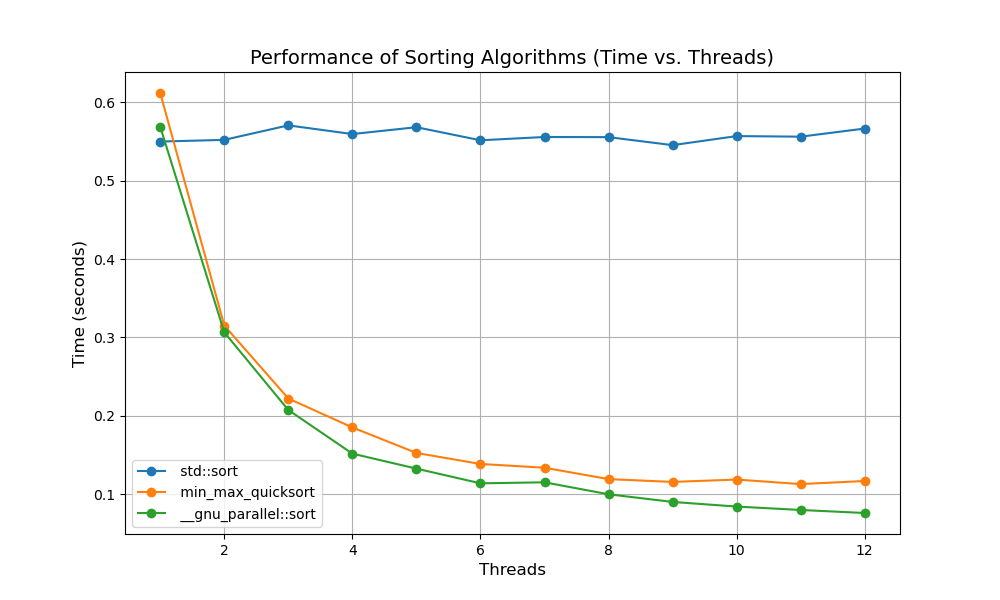
\includegraphics[width=\linewidth]{./running_times.png}

~\\
And here are the performance gains compared to std::sort():

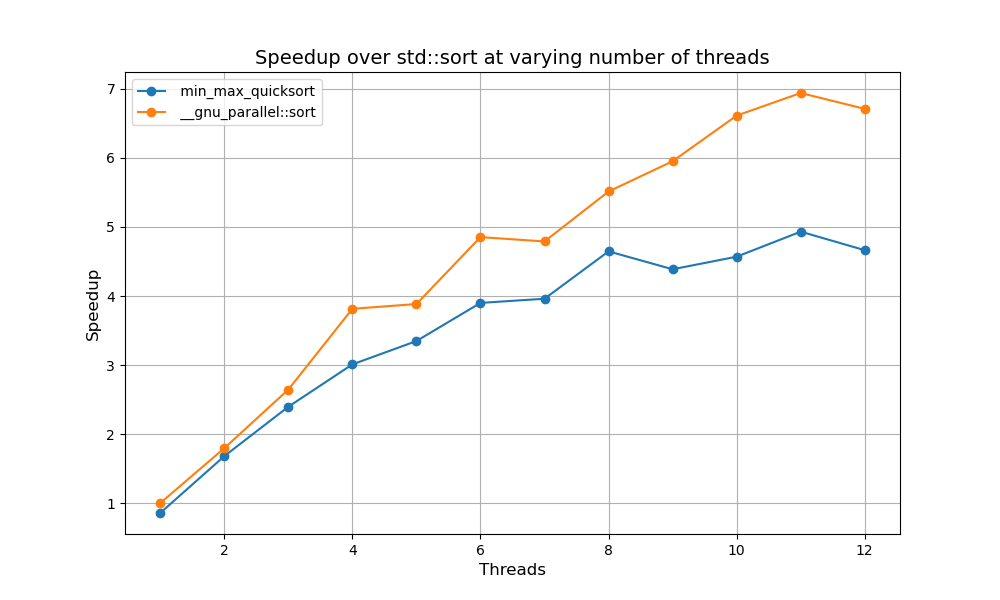
\includegraphics[width=\linewidth]{./speedup.png}


\newpage
\subsubsection{Running time comparison with different array sizes}
Here are the running times with varying array sizes:

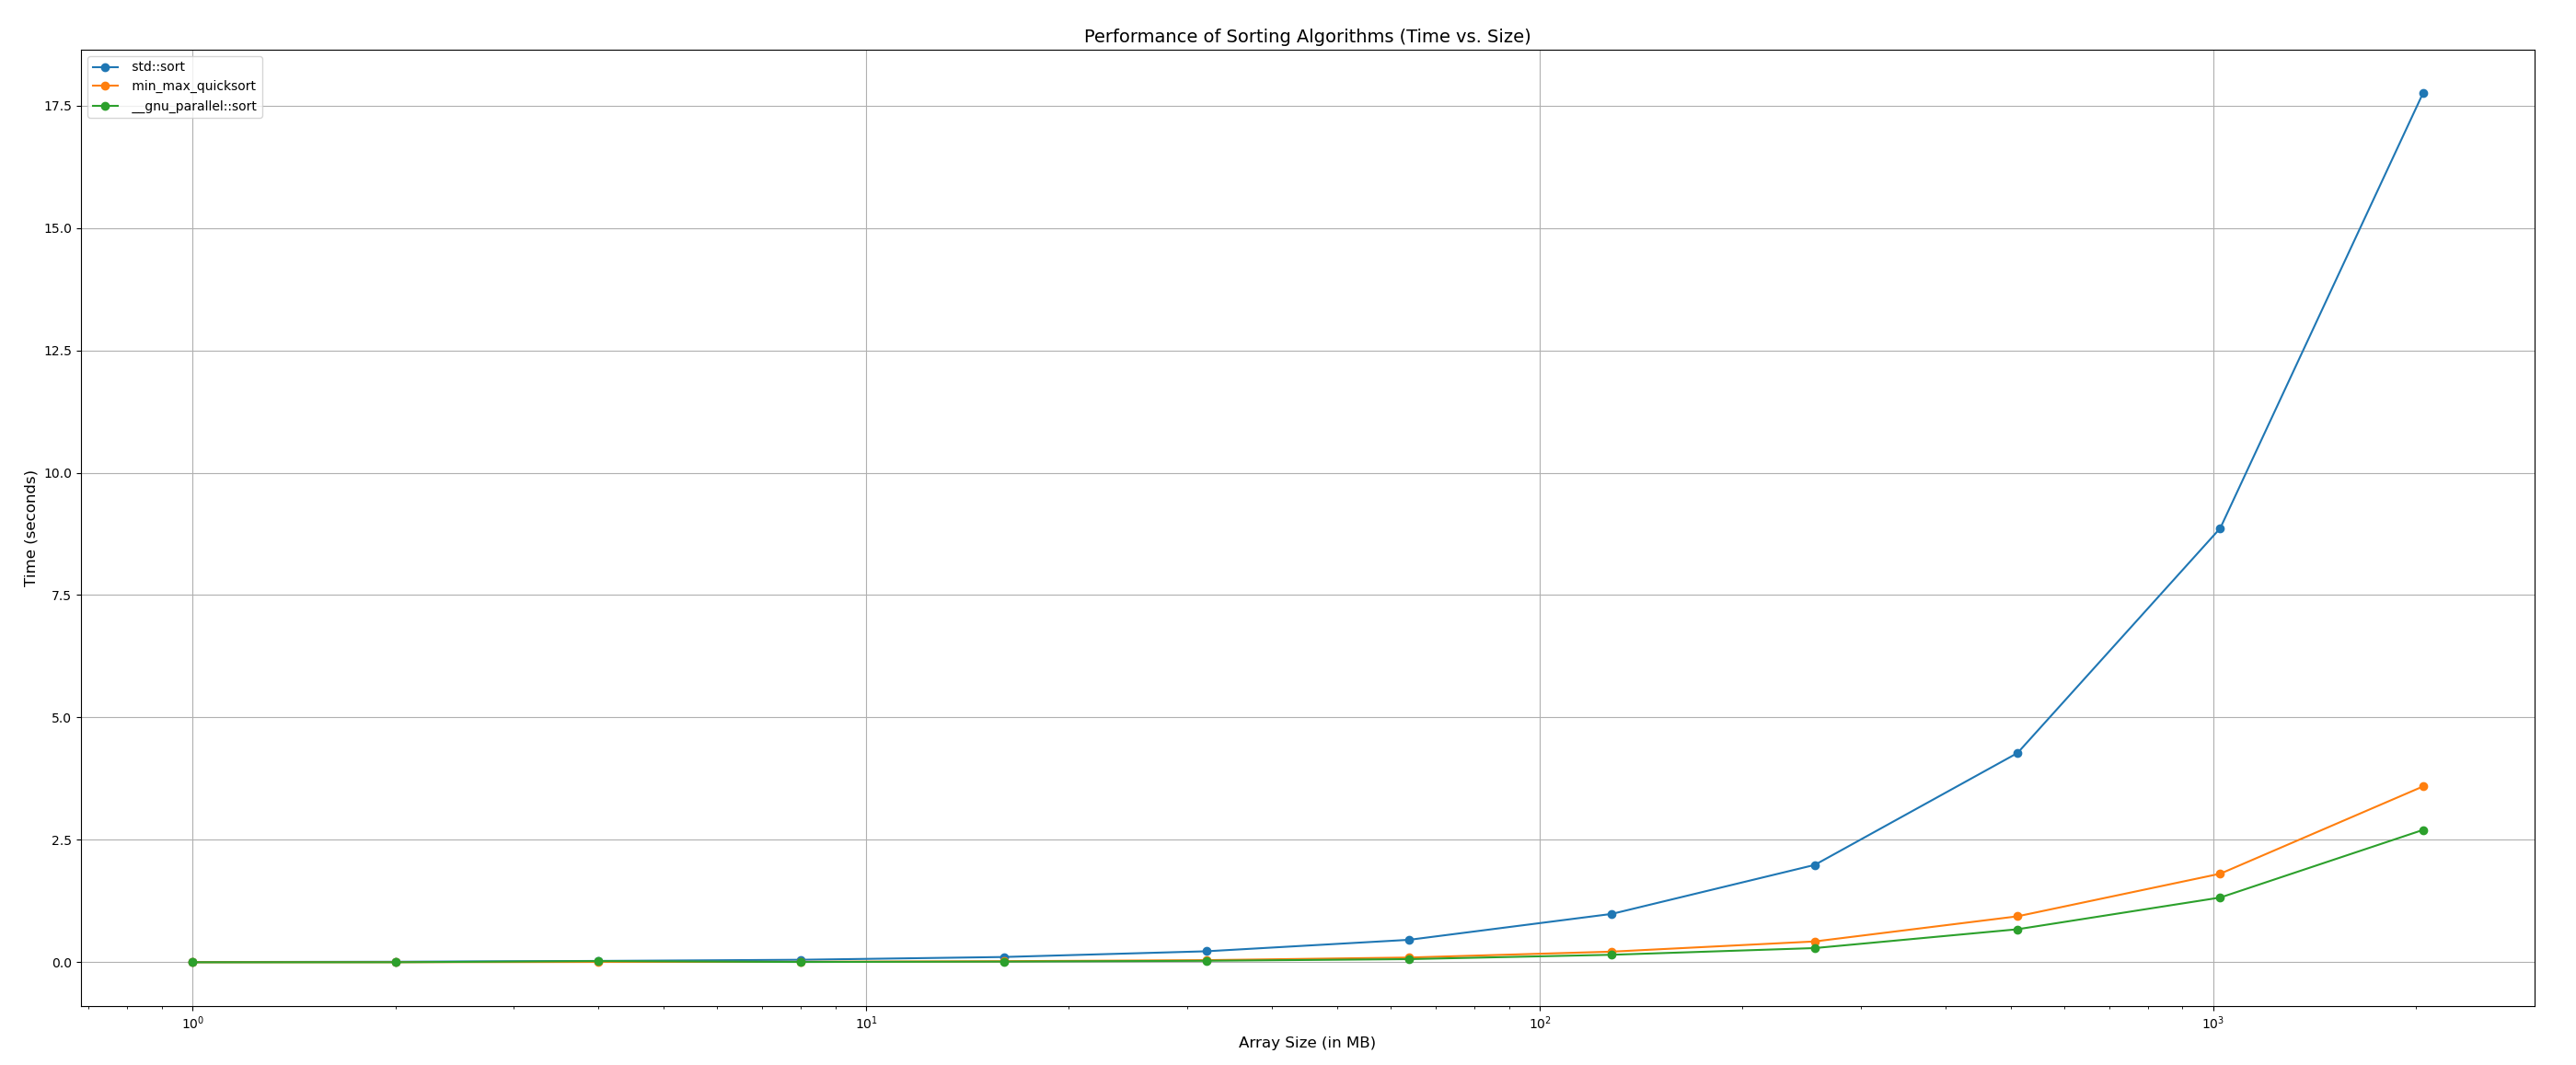
\includegraphics[width=\linewidth]{./running_times_array.png}

~\\
These are the speedups compared to std::sort():

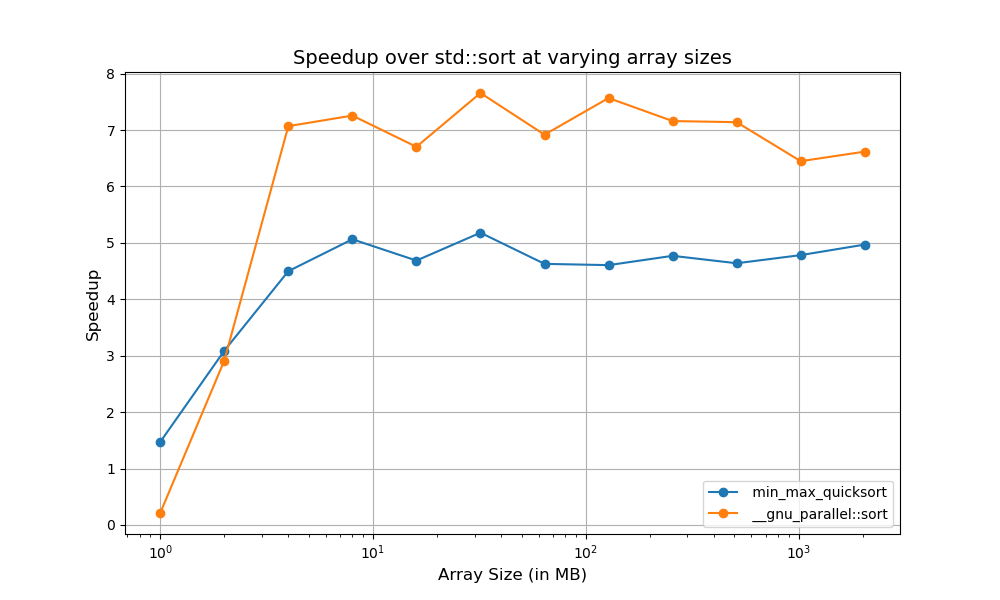
\includegraphics[width=\linewidth]{./speedup_array.png}


~\\
\subsubsection{Explaining the results}
In the first two graphs when measuring the running times and speed ups when varying the threads, we can clearly see that the serial std::sort has a constant running time, whereas both parallel sorting algorithms run quicker with increasing thread number, thus overtaking std::sort already with two threads significantly (almost halving the running time of std::sort).
With further increasing thread number, the running times of the parallel algorithms further decreases.
They are proportional to $\frac{1}{\text{Number of Threads}}$, as one might expect, but the proportionality factor is roughly at 2, meaning there is quite some overhead compared to the optimal running time of $\frac{\text{Serial Running Time}}{\text{Number of Threads}}$.

\bigskip

~\\
% Let us now analyze the second two pictures, showing the running times at different array sizes.
% The graphs are as expected, the running times of the parallel algorithms is better, even more so for very large array sizes, as in those instances we can fully employ the parallel power of the cpu cores, thus decreasing the running time significantly.
% This is why the speedup gets better with increasing array size.
% One might think that this speedup is exponential, but it is not (note the logarithmic scale!), it is rather approximately $(\text{Serial Running Time}) \cdot (1 - \frac{1}{12 \cdot E})$, where $E$ is the efficiency $E = \frac{\frac{\text{Serial Running Time}}{\text{Threads}}}{\text{Parallel Running Time}}$, and note that the number of threads on this machine is 12.
% Note, that Serial Running Time is expected to grow $\Theta(n \cdot \log(n))$, and so should the speedup.
Let us now analyze the second two pictures, showing the running times at different array sizes.
The graphs are as expected, the running times of the parallel algorithms is better, even more so for very large array sizes, as in those instances we can fully employ the parallel power of the cpu cores without much overhead relative to the running time, thus decreasing the running time significantly.
This is why the speedup gets better with increasing array size initially.
The speedup, however, start to plateau quickly at an array size of roughly 1 MB, as at this point the overhead of parallelization with respect to the running time stays constant (i.e. $\frac{\text{Time of Overhead}}{\text{Parallel Running Time}} = \text{const.}$):

~\\
Since
\[
    \text{speedup} = \frac{\text{Serial Running Time}}{\text{Parallel Running Time}} \ \ \ \ \ ,
\]
and
\begin{align*}
    \text{Parallel Running Time} &= \frac{\text{Serial Running Time}}{\text{Number of Threads}} + \text{Time of Overhead} \\ \\
    &= \frac{\text{Serial Running Time}}{\text{Number of Threads}} + \alpha \cdot \text{Parallel Running Time} \\ \\
    % \frac{\text{Time of Overhead}}{\text{Parallel Running Time}} \\
    &= \frac{\frac{\text{Serial Running Time}}{Number of Threads}}{1-\alpha} \\ \\
    &= \alpha' \cdot \text{Serial Running Time} \ \ \ \ \ ,
\end{align*}
we have
\[
    \text{speedup} = \frac{1}{\alpha'} = \text{const.} \ \ \ \ \ .
\]

% One might think that this speedup is exponential, but it is not (note the logarithmic scale!), it is rather approximately $(\text{Serial Running Time}) \cdot (1 - \frac{1}{12 \cdot E})$, where $E$ is the efficiency $E = \frac{\frac{\text{Serial Running Time}}{\text{Threads}}}{\text{Parallel Running Time}}$, and note that the number of threads on this machine is 12.
% Note, that Serial Running Time is expected to grow $\Theta(n \cdot \log(n))$, and so should the speedup.

\newpage
\subsection{What every systems programmer should know about concurrency}
\subsubsection{Why it is not enough to declare shared variables as volatile}
By declaring variables as volatile in C and C++, we make the compiler read and write the variable from and to memory every time we access it.
Cache coherency protocols then ensure that every local cache of the cpu cores has the same value of the shared variable.
So everything should be good then, right?

~\\
Well, there is one problem: Modifying the shared variable isn't an atomic operation.
Imagine two threads wanting to increment a shared counter.
But as executing this increment operation takes multiple clock cycles, thread one starts reading the counter from memory, and a few ticks later thread two reads the same value of memory.
Now, both threads increment this value and write it back to memory, so thread one does it first, which causes the cache of thread two to now have the updated counter variable in its cache, but the value it is operating on, which lies in its registers, is unchanged, so it will get the same result and write it back to memory.
In the end, the counter increased by one, even though it got incremented two times, which is (in most cases) undesired and incorrect behavior.

~\\
\subsubsection{But what if my ISA doesn't support atomic access to my custom data structure / code section}
We now learned that we have to use atomic variables to ensure correct parallel code execution.
But what if the shared variable has no atomic variable data type like bool has with std::atomic\_bool?
Or we want to synchronize an entire code section?
As it turns out, we only need a few of these atomic operations and data types to implement generic synchronization functionality, as those can be used to built so called \em locks\em . 

~\\
One well known example is a \em semaphore\em . It basically consists of an atomic counter, which represents how many threads may still access the shared resource (it is mostly either 0 or 1).
If two threads want to access a shared resource, they have to first check if the semaphore has a value of one, and only if it does, decrement the value immediately and progress in their execution.
If the semaphore is zero, the thread has to wait (which is mostly done by making it sleep).
As you can see, "check if semaphore is one, and if so decrement it" must be an atomic operation for the semaphore to work.
And this is exactly why modern ISA have instructions like \em compare-and-swap\em , which implement such operations atomically in hardware.
There are also some other common instructions of this kind. They are combined under the term \em read-modify-write\em .
\end{document}